\documentclass[conference]{IEEEtran}
\IEEEoverridecommandlockouts
% The preceding line is only needed to identify funding in the first footnote. If that is unneeded, please comment it out.
%Template version as of 6/27/2024

\usepackage{amsmath,amssymb,amsfonts}
\usepackage{algorithmic}
\usepackage{graphicx}
\usepackage{textcomp}
\usepackage{xcolor}
\usepackage[backend=biber,style=numeric]{biblatex}
\addbibresource{report.bib}

 \graphicspath{{assets/latex/}}

\begin{document}

\title{CS6524 Computer Vision Lab. 1\\ Silhouettes and Fourier Epicycles}

\author{\IEEEauthorblockN{Patrick Walsh}
\and
\IEEEauthorblockN{Dara Heaphy}
\and
\IEEEauthorblockN{Tiernan Scully}
}

\maketitle

\begin{abstract}
We extract an animal's outline from a single image so that it can be redrawn with Fourier epicycles. Our first version followed the suggested pipeline with one threshold for every image, and it failed on four of our six images. Choosing a threshold per image fixed two of those four. The giraffe and tiger stayed poor because no threshold could keep their pale parts without also picking up the ground.
\end{abstract}

\section{Introduction}
The brief gives a pipeline of grayscale conversion, blurring, thresholding and border detection, and says it may not suit every image. We treated it as a starting point: we ran it as given, looked at where it broke, and only then decided what to change. This report follows that order. Our six test images are illustrations of a duck, buffalo, fish, giraffe, squid and tiger.

\section{Method}

\subsection{From image to border}
Each image is converted to grayscale with equal channel weights of 0.333 and then blurred with a Gaussian kernel~\cite{foundationsCVbook},
\begin{equation}
G(x,y) \propto \exp\!\left(-\frac{x^2+y^2}{2\sigma^2}\right),
\label{eq:gaussian}
\end{equation}
normalised to sum to one. The kernel radius is $\lceil 3\sigma \rceil$, so $\sigma=2$ gives a $13\times13$ kernel. We reflect the image at its borders so that the white background does not darken or brighten near the edges.

All of our animals are darker than their backgrounds, so the mask keeps pixels below a threshold $T$:
\begin{equation}
M(x,y) = I_\sigma(x,y) < T.
\label{eq:threshold}
\end{equation}
Text and watermarks also pass this test, so we keep only the largest 8-connected region. Interior holes are then filled by flooding the background inward from outside the image; anything the flood cannot reach becomes foreground.

The border comes from Sobel filters applied to the mask:
\begin{equation}
S_x = \frac{1}{8}\begin{bmatrix}-1&0&1\\-2&0&2\\-1&0&1\end{bmatrix},\quad
S_y = S_x^{\top}.
\label{eq:sobel}
\end{equation}
Sobel responds on both sides of an edge, which gives a line about two pixels thick. Tracing needs one pixel, so we keep a pixel only if its gradient magnitude exceeds 0.1, it is foreground, and at least one of its 4-neighbours is background. Fig.~\ref{fig:pipeline} shows each stage on the fish.

\begin{figure}[t]
\centerline{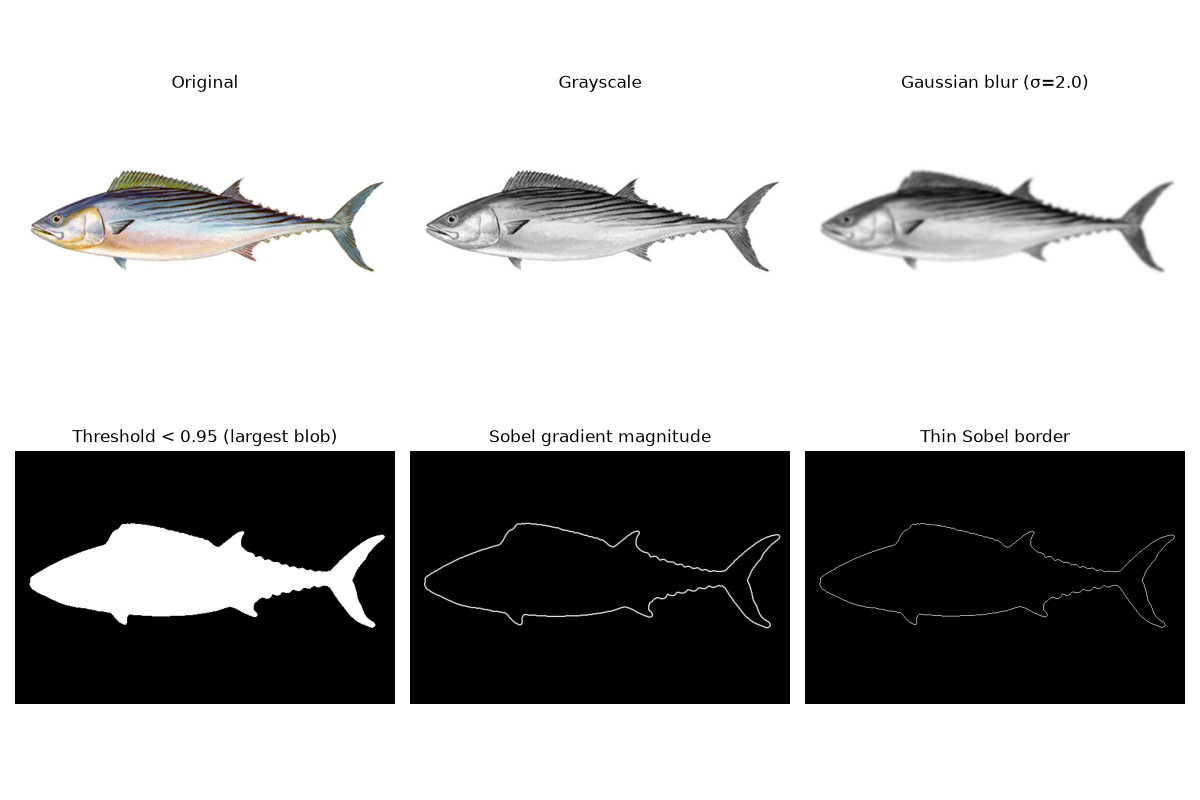
\includegraphics[width=\columnwidth]{pipeline_fish.png}}
\caption{Each pipeline stage on the fish at $T=0.95$, our cleanest result.}
\label{fig:pipeline}
\end{figure}

\subsection{From border to trajectory}
We walk the border with Moore neighbour tracing, which visits pixels in the order they appear along the outline. The brief's nearest-neighbour snippet can jump across the shape and leave straight lines through it, and following the contour avoids those jumps. We then resample to $N=500$ points at equal arc length. The endpoint is left out so the first point is not repeated, because the samples will be treated as one period of a signal.

\subsection{Fourier descriptors}
This stage is not implemented yet. The trajectory will become the complex signal $z[n]=x[n]+iy[n]$, and reconstruction will keep the set $\mathcal{S}_K$ of the $K$ largest coefficients of its DFT $Z[u]$:
\begin{equation}
z'[n] = \frac{1}{N}\sum_{u\in\mathcal{S}_K} Z[u]\,e^{2\pi i u n/N}.
\label{eq:fourier}
\end{equation}

\section{Choosing the threshold}
Our first configuration used $T=0.5$ and $\sigma=2$ for every image. That value only caught the darkest parts of the lighter animals: the mask covered 1\% of the giraffe image, 2\% of the squid, 5\% of the fish and 7\% of the tiger. The giraffe's mask was a thin strip along its neck and back.

The obvious first change was the threshold, so we swept $T$ from 0.5 to 0.95 with everything else fixed (Fig.~\ref{fig:sweep}). We chose each value by inspecting the masks, and Table~\ref{tab:thresholds} gives the results.

\begin{figure}[t]
\centerline{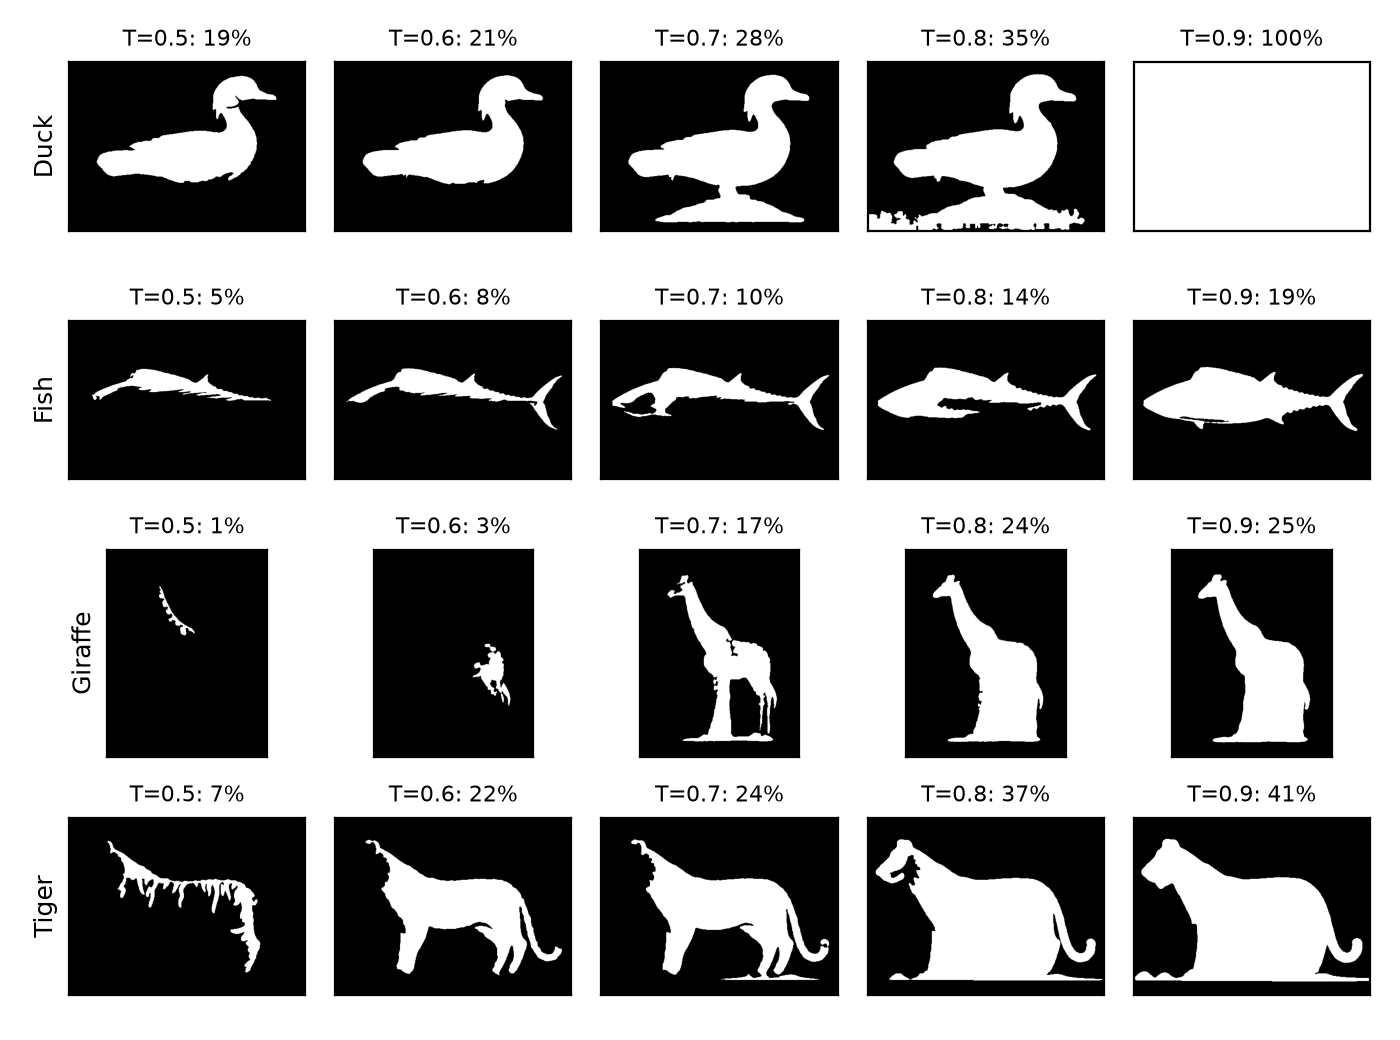
\includegraphics[width=\columnwidth]{threshold_sweep.png}}
\caption{Masks at increasing $T$ with $\sigma=2$, with the share of the image each one covers. The all-white duck panel at $T=0.9$ is the paper flooding the mask.}
\label{fig:sweep}
\end{figure}

\begin{table}[t]
\caption{Chosen threshold for each image}
\begin{center}
\begin{tabular}{|l|c|l|}
\hline
\textbf{Image} & $\boldsymbol{T}$ & \textbf{Result} \\
\hline
Duck & 0.7 & Legs kept; mound still attached \\
Buffalo & 0.8 & Horn and tail recovered \\
Fish & 0.95 & Whole fish \\
Squid & 0.8 & Body and tentacles \\
Giraffe & 0.7 & Rough outline; legs merge with ground \\
Tiger & 0.7 & Face missing; ground attached \\
\hline
\end{tabular}
\label{tab:thresholds}
\end{center}
\end{table}

Mask area turned out to be a quick way to read the sweep, because sudden jumps show where a threshold stops working. The fish grows steadily from 5\% to 20\% as its pale belly joins the body. The duck goes from 35\% at $T=0.8$ to 100\% at $T=0.9$, because its cream paper is darker than the white backgrounds of the other images and falls below the threshold. A value that suits the fish therefore destroys the duck, which is why one global value could not work.

\section{Discussion}
Tuning $T$ gave usable outlines for four images, but the giraffe and tiger show its limit. The tiger's mask jumps from 24\% to 37\% between $T=0.7$ and $T=0.8$. At 0.7 the face is missing. At 0.8 the face appears, but the ground fuses to the feet, the space between the legs becomes an enclosed hole, and hole filling turns the legs into a solid block. The giraffe's ground shadow does the same thing to its legs.

These look like one failure but we think there are two causes. The tiger's face and the background are both bright, and grayscale has already discarded the colour that might tell them apart, so this is a problem with what the pixels measure. The ground is different: it is genuinely darker than the background and touches the animal, so it is a problem of shape and connectivity that a better pixel measure may not solve. We plan to address them separately, starting with colour.

Our sweep also has limits. We picked $T$ by eye, so the values are not reproducible by any rule, and we held $\sigma$ fixed, so we do not yet know how much blur affects these results.


\printbibliography

\end{document}
